% Copy to docs/ambiguities/lectureNN/main.tex when actual questions arise.
% Replace NN and the title; add real LNN-Qxx entries from the lecture ledger.
% Build from the repository root: make questions LECTURE=NN
% Store evidence crops in the new project's images/ folder.
% Questions are for later review. Do not stop transcription or ask live chat
% questions; deliver this PDF with the lecture, keeping unresolved items marked.
\documentclass[a4paper,12pt]{article}
\usepackage[margin=19mm]{geometry}
\usepackage{amsmath,amssymb,graphicx,xcolor}
\usepackage{fontspec}
\usepackage{url}
\usepackage{xepersian}
\settextfont{XB Roya}
\setlatintextfont{Latin Modern Roman}
\definecolor{ink}{HTML}{173D75}
\graphicspath{{images/}}
\setlength{\parindent}{0pt}
\setlength{\parskip}{5pt}
\linespread{1.12}
\newcommand{\qtitle}[2]{{\Large\bfseries\color{ink} پرسش \lr{#1}: #2}\par}
\newcommand{\answer}{\medskip\textbf{پاسخ یا صورت مورد تأیید و تاریخ:}\par\vspace{18mm}\hrule\medskip}
\begin{document}
{\LARGE\bfseries پرسش‌های ابهام جلسهٔ \lr{15}}\par
{\large جزوهٔ جبر پیشرفتهٔ دکتر خسروی}\par
صفحه‌ها یک‌مبنا و مربوط به فایل پی‌دی‌اف‌اند. هر سه پرسش باز هستند؛ پاسخ کاربر تا تاریخ \lr{2026-10-25} ثبت نشده است. رونویسی با انتخاب‌های موقت پایان می‌یابد.
\medskip\hrule\medskip
\qtitle{L15-Q01}{نسخهٔ مبنا و بخش افزوده}
\textbf{وضعیت:} باز؛ ترتیب نسخهٔ \lr{unresolved-a} موقت است.\par
\textbf{نشانی منبع:} کل دو سند، به‌ویژه صفحهٔ ۱۳ و پایان آن‌ها:
\begin{LTR}\footnotesize
\texttt{sources/lectures/15 Jacobson Radical.pdf} (unresolved-a; 16 pages)\\
\texttt{sources/lectures/15 Jacobson Radical\_241111\_015647.pdf} (unresolved-b; 13 pages)
\end{LTR}
\textbf{نتیجهٔ مقایسه:} صفحات ۱ تا ۱۲ دو نسخه از نظر محتوای ریاضی متناظرند. نسخهٔ نخست در صفحهٔ ۲ یادداشت قرمز دربارهٔ مدول بودن \(R/I\) و در صفحات ۱۰ و ۱۱ تأکیدهای حاشیه‌ای دارد. صفحهٔ ۱۳ نسخهٔ دوم تنها صورت قضیهٔ هاپکینز--لویتسکی را دارد؛ ادامهٔ صفحهٔ ۱۳ نسخهٔ نخست و صفحات ۱۴ تا ۱۶ آن، اثبات و نتایج را اضافه می‌کنند. محتوای ریاضیِ منحصر به نسخهٔ دوم یا جایگزین متعارض یافت نشد.\par
\textbf{شاهد:} آغاز صفحهٔ ۱۳ نسخهٔ نخست در چپ و صفحهٔ ۱۳ نسخهٔ دوم در راست:
\begin{center}
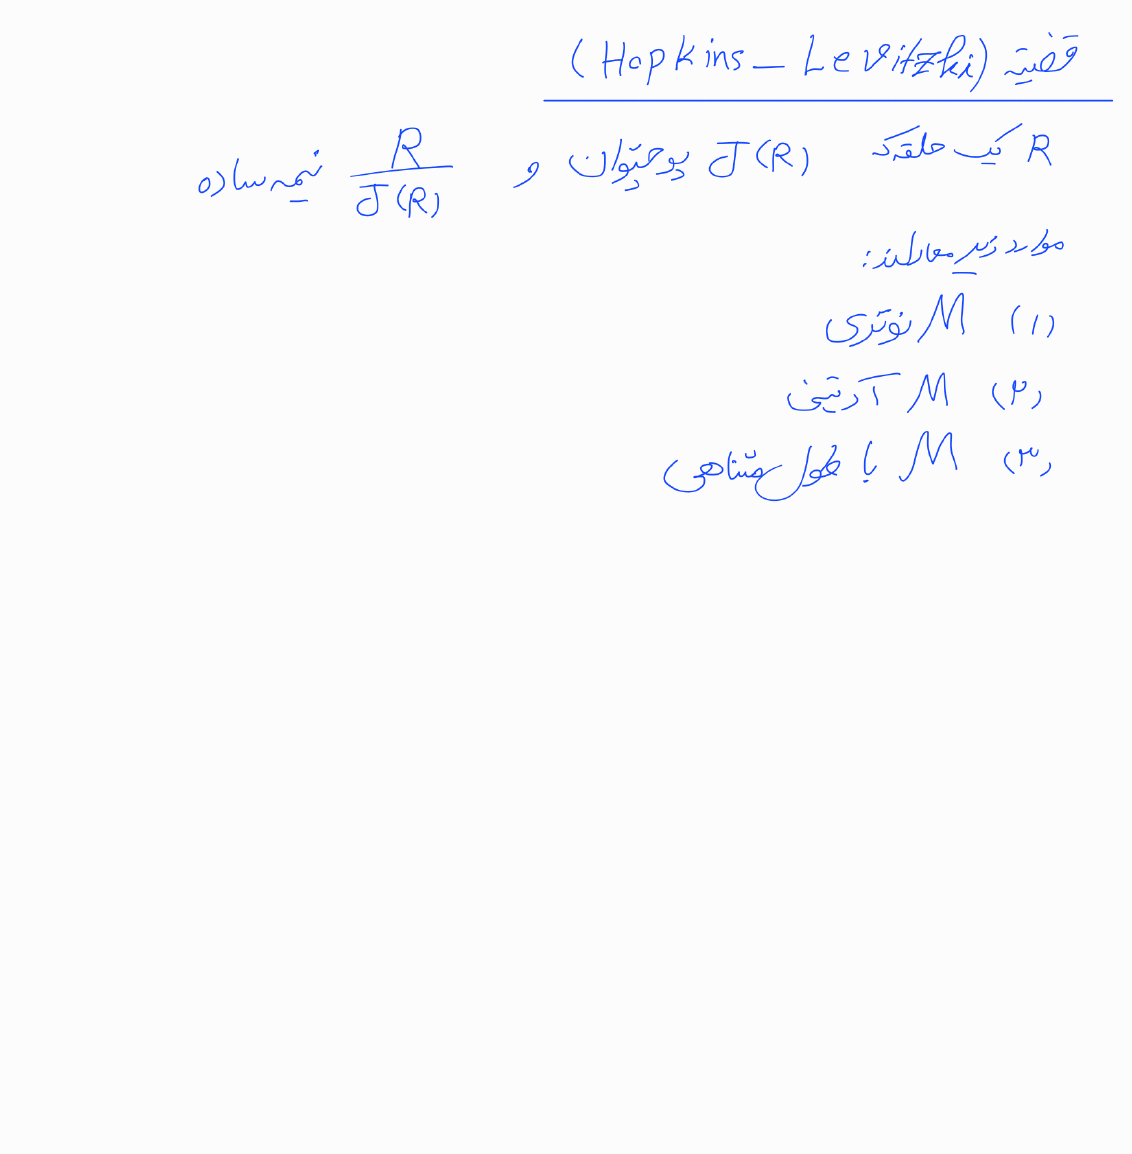
\includegraphics[width=.46\linewidth,height=48mm,keepaspectratio]{variant-b13.png}\hfill
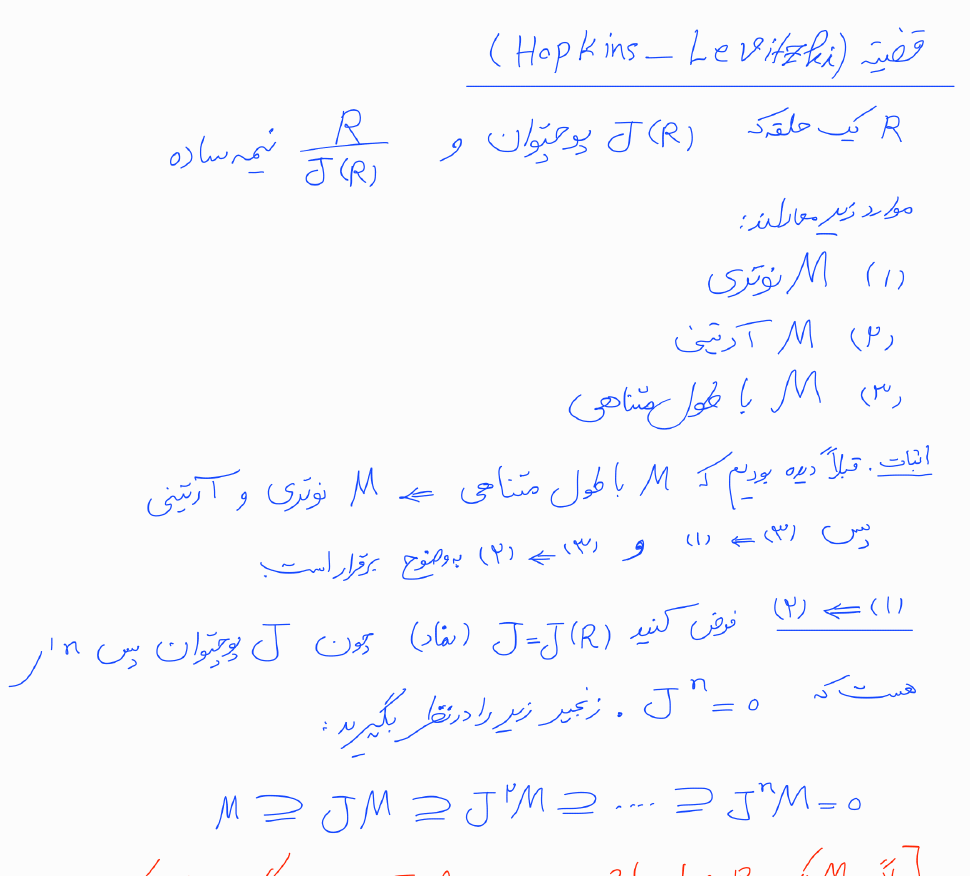
\includegraphics[width=.46\linewidth,height=48mm,keepaspectratio]{variant-a13.png}
\end{center}
\textbf{گزینه‌ها و اثر:} نسخهٔ نخست می‌تواند نسخهٔ مفصل‌تر باشد، یا نسخهٔ دوم عمداً کوتاه‌تر باشد. تطابق محتوا، به‌تنهایی مرجع بودنِ هیچ‌کدام را ثابت نمی‌کند. حذف ادامهٔ نسخهٔ نخست، اثبات قضیه و نتایج پایانی را حذف می‌کند.\par
\textbf{پرسش:} کدام نسخه مرجع نهایی است و آیا اثبات و نتایج افزودهٔ نسخهٔ نخست باید حفظ شوند؟\par
\textbf{انتخاب موقت:} ترتیب ۱۶صفحه‌ای نسخهٔ نخست و همهٔ مطالب افزوده حفظ شده؛ اصالت نسخه تعیین نشده است.
\answer
\newpage
\qtitle{L15-Q02}{دو توان ناسازگار در اثبات هاپکینز--لویتسکی}
\textbf{وضعیت:} باز؛ دو جایگزینیِ پیشنهادی در اسلاید به‌صراحت موقت‌اند.\par
\textbf{نشانی منبع:} نسخهٔ \lr{unresolved-a}، صفحهٔ ۱۴، زنجیر سری ترکیبی در نیمهٔ میانی و همریختی بلافاصله زیر آن. این اثبات در نسخهٔ دوم وجود ندارد.
\begin{LTR}\footnotesize\texttt{sources/lectures/15 Jacobson Radical.pdf}\end{LTR}
\textbf{عبارت‌های دیده‌شده:}
\[
 0=\frac{J^kM}{J^{k+1}M},\qquad
 \frac{M_{t+1}/J^{k+1}M}{M_t/J^kM}\cong\frac{M_{t+1}}{M_t}.
\]
\begin{center}
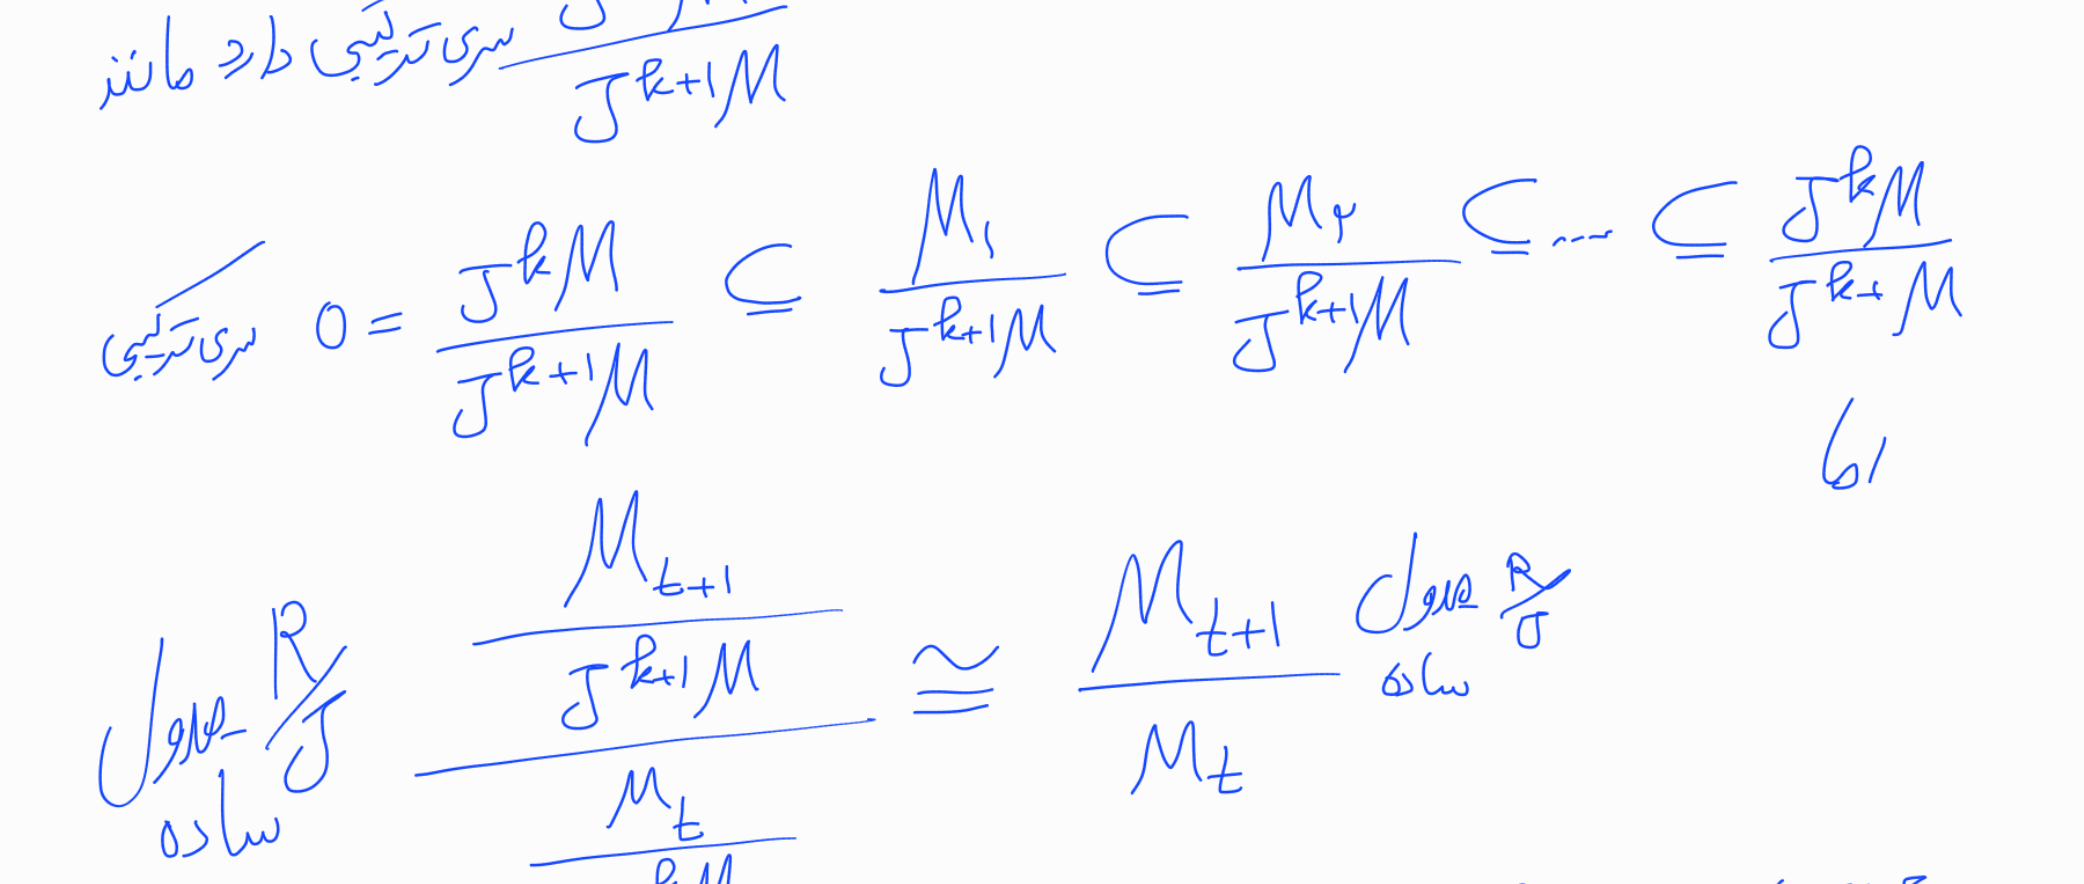
\includegraphics[width=.94\linewidth,height=47mm,keepaspectratio]{a14-chain.png}\\[2mm]
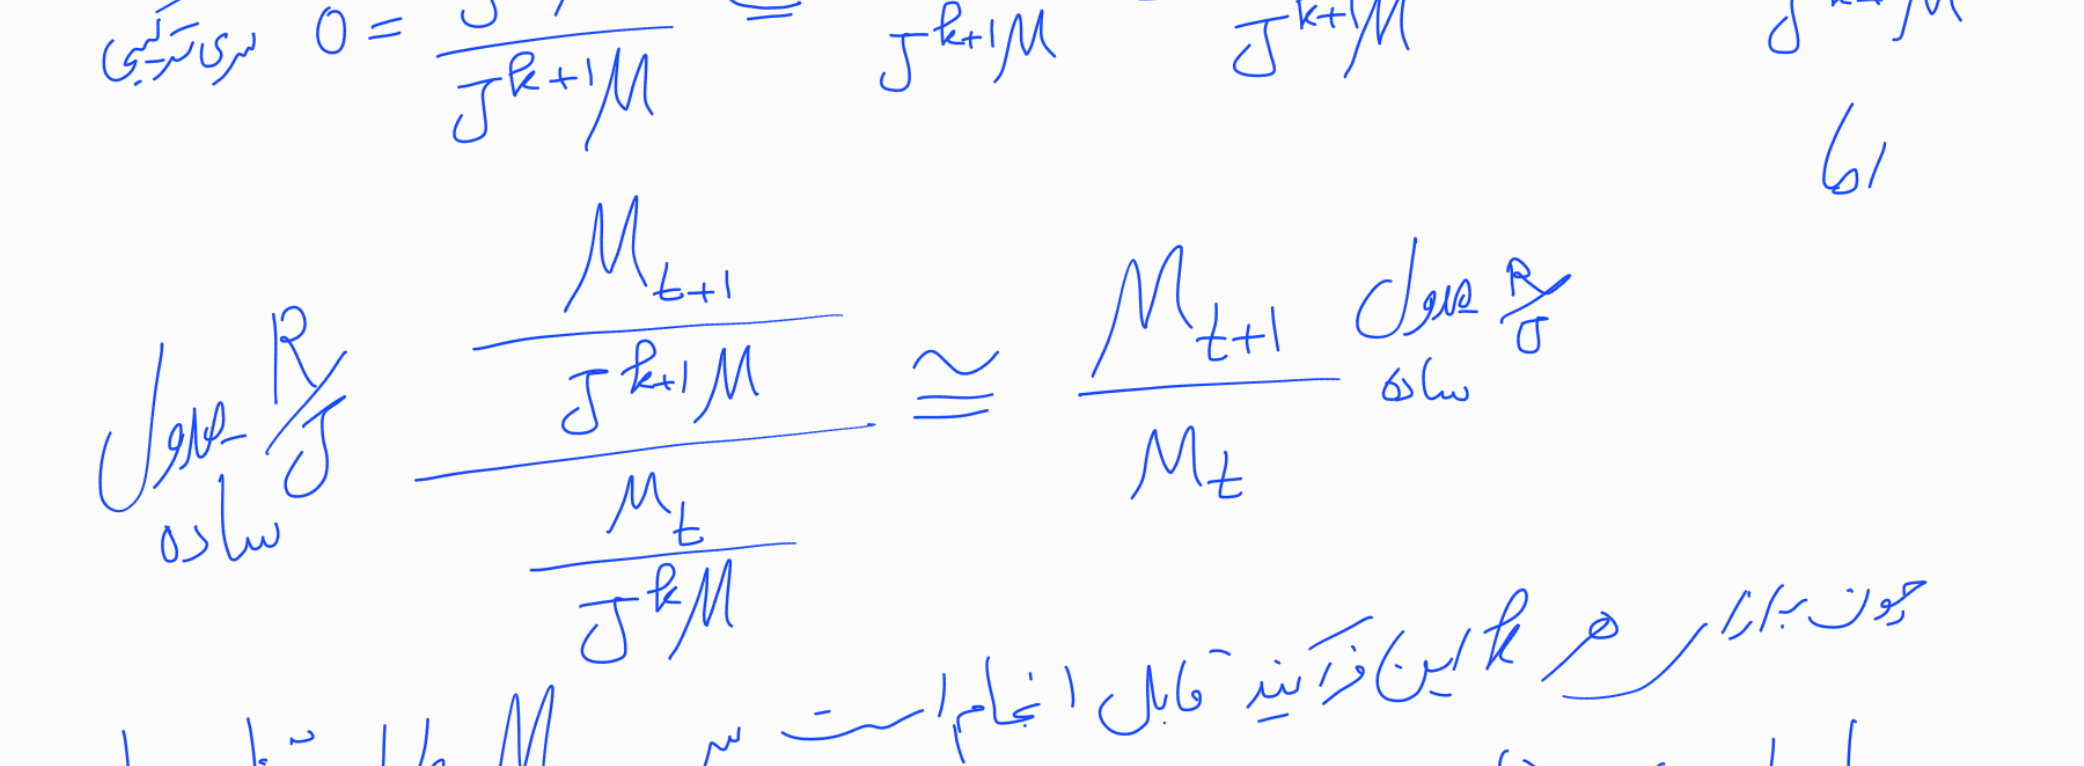
\includegraphics[width=.94\linewidth,height=43mm,keepaspectratio]{a14-isomorphism.png}
\end{center}
\textbf{خوانش‌ها:} می‌توان توان‌های نوشته‌شده را عیناً نگه داشت؛ یا در صورتِ جملهٔ صفر و در مخرجِ خارج‌قسمتِ پایین، \(k\) را به \(k+1\) تبدیل کرد.\par
\textbf{اثر:} \(J^kM/J^{k+1}M\) عموماً صفر نیست؛ همچنین برای قضیهٔ سوم همریختی، دو خارج‌قسمت باید بر یک زیرمدول مشترک باشند. صورتِ پیشنهادی چنین است:
\[
 0=\frac{J^{k+1}M}{J^{k+1}M},\qquad
 \frac{M_{t+1}/J^{k+1}M}{M_t/J^{k+1}M}\cong\frac{M_{t+1}}{M_t}.
\]
\textbf{پرسش:} آیا در هر دو موضع، توانِ مورد نظر \(k+1\) است؟\par
\textbf{انتخاب موقت:} دو فرمولِ پیشنهادی در قاب \lr{lec15:lift-composition-series} با هشدارِ خوانش موقت آمده‌اند؛ متن لفظی در این صفحه محفوظ است.
\answer
\newpage
\qtitle{L15-Q03}{زیرنویسِ پرسش حلقهٔ ماتریسی}
\textbf{وضعیت:} باز؛ زیرنویس دوم بدون تأیید به راست تبدیل نشده است.\par
\textbf{نشانی منبع:} هر دو نسخه، صفحهٔ ۱، سطر «سؤال» نزدیک پایین صفحه. پرسشِ صفحهٔ ۴ تنها رادیکال چپ را می‌نویسد.
\begin{LTR}\footnotesize
\texttt{sources/lectures/15 Jacobson Radical.pdf} (unresolved-a)\\
\texttt{sources/lectures/15 Jacobson Radical\_241111\_015647.pdf} (unresolved-b)
\end{LTR}
\textbf{خوانش لفظیِ شاهد:}
\[
 J_\ell(M_n(D))=J_\ell(M_n(D))=?
\]
\begin{center}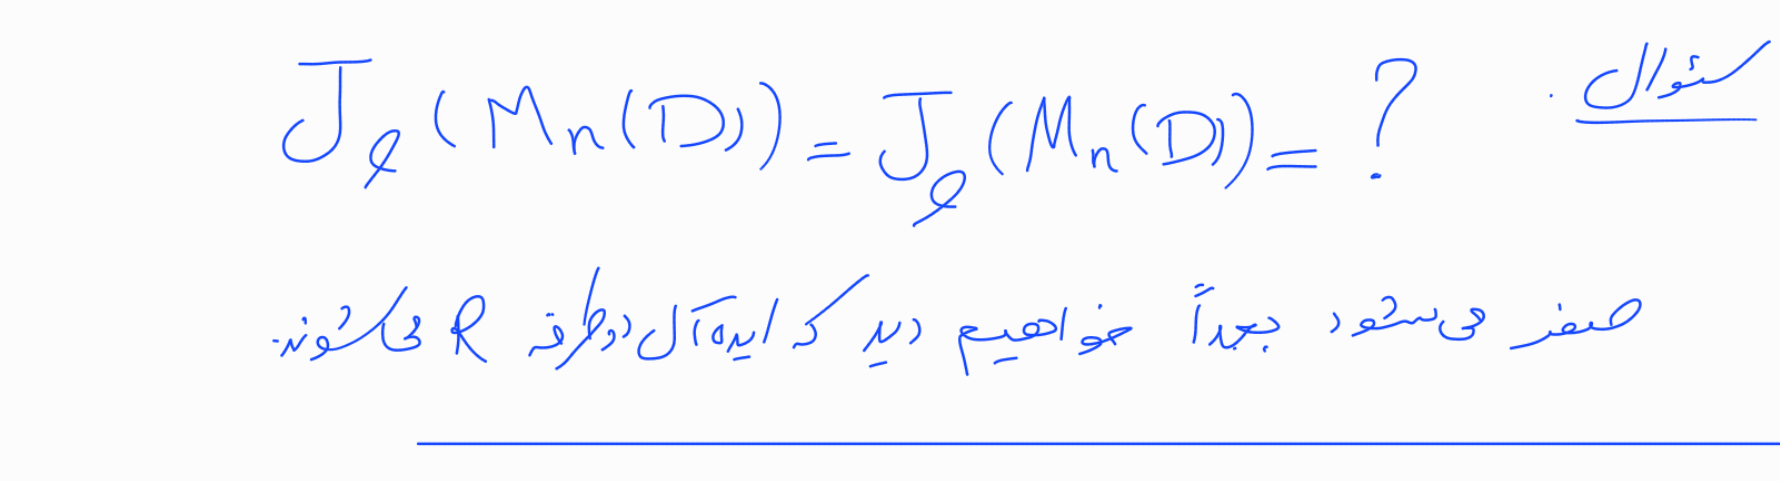
\includegraphics[width=\linewidth]{matrix-question.png}\end{center}
\textbf{خوانش‌های ممکن:} تکرار عمدیِ \(J_\ell\)، یا لغزش قلم به جای \(J_r\) در یکی از دو طرف.\par
\textbf{اثر:} خوانش نخست فقط یک کمیت را می‌پرسد؛ خوانش دوم هر دو رادیکال را مطرح می‌کند. بعدتر در صفحهٔ ۹، برابری عمومی رادیکال‌های چپ و راست آمده است، اما آن نتیجه، زیرنویس لفظیِ این سطر را تعیین نمی‌کند.\par
\textbf{پرسش:} آیا یکی از دو زیرنویسِ این سطر باید \(r\) باشد؟\par
\textbf{انتخاب موقت:} پرسش به صورت «رادیکال حلقهٔ \(M_n(D)\) چیست؟» حفظ شده و هشدارِ زیرنویس در قاب \lr{lec15:radical-examples} آمده است. استفادهٔ بعدیِ جزوه از \(J_\ell(M_n(D))=0\) در اثبات نیمه‌سادگی، مستقل از این سؤالِ نگارشی حفظ شده است.
\answer
\end{document}
